% Standalone native LaTeX framework. The prior main.tex manuscript is preserved.
\documentclass[11pt,a4paper]{article}
\usepackage[margin=0.9in]{geometry}
\usepackage[T1]{fontenc}
\usepackage{lmodern,amsmath,amssymb,graphicx,booktabs,tabularx,array}
\usepackage[round,authoryear]{natbib}
\usepackage[section]{placeins}
\usepackage{xurl}
\usepackage[colorlinks=true,linkcolor=blue,citecolor=blue,urlcolor=blue]{hyperref}
\setlength{\emergencystretch}{2em}
\setlength{\parskip}{0.2em}
\setlength{\tabcolsep}{4pt}
\renewcommand{\arraystretch}{1.13}
\renewcommand{\topfraction}{0.95}
\renewcommand{\bottomfraction}{0.9}
\renewcommand{\textfraction}{0.05}
\renewcommand{\floatpagefraction}{0.8}
\raggedbottom
\hypersetup{pdftitle={CF-MoA: Taxonomy-Guided Benchmarking and Agent Orchestration for Counterfactual Medical Reasoning},pdflang={en}}
\title{CF-MoA: Taxonomy-Guided Benchmarking and Agent Orchestration for Counterfactual Medical Reasoning\\[0.6em]\large Complete paper framework and verified evidence map}
\author{}
\date{3 October 2026}
\begin{document}
\maketitle
\noindent\textbf{Document status.} This is the proposed paper structure, with a candidate abstract, contribution statements, section-level arguments, and verified results selected from completed experiments. It precedes a full rewrite of the earlier manuscript. No new model inference or grading was performed for this document. Historical results and unsuccessful extensions remain available in the evidence package.

\begin{abstract}
Medical question answering under changed conditions requires both revising affected judgments and preserving unaffected ones. Existing medical counterfactual and perturbation resources offer diverse tasks, but their dataset boundaries do not provide a common account of these functional requirements. We introduce a five-category taxonomy covering support establishment, support withdrawal, candidate re-comparison, consequence derivation, and judgment preservation. An auditable collection and qualification process traces 55,991 archived comparison records from 15 acquired resources to an evaluation benchmark containing 6,104 units and 13,000 selected judgments from 11 sources, while retaining original questions and native scoring. Evaluation of seven medical question-answering configurations exposes substantial weaknesses on support-changing and candidate-comparison subsets. We develop corresponding specialized capabilities and organize them as Counterfactual Mixture of Agents (CF-MoA), a five-operation framework with capability-based routing and native answer readout. Its adopted sparse instantiation improves full-benchmark native scores by 10.09 and 12.01 percentage points on two backbones, while improving both response and preservation pair correctness. Terminal-head experiments produce positive gains in all 21 configuration-by-category comparisons across three categories. Operation-level controls clarify which benefits arise from support recomputation, candidate accessibility, or answer aggregation. These exposed-development results support functional organization as a useful approach to benchmarking and improving medical counterfactual systems.
\end{abstract}

\section{Central Argument and Contributions}
The paper should connect the way counterfactual tasks are organized to the way a system processes their evidence. A change can establish support, invalidate support, alter a ranking, propagate through an explicit model, or leave a target unaffected. These requirements motivate both the annotation scheme and the five operational roles. Their relationship is functional: offline category membership is not supplied to the online router.

The proposed contributions are:
\begin{enumerate}
\item \textbf{A functional taxonomy.} Five target-specific relations describe what a change demands of a judgment. Overlapping labels retain cases involving multiple relations, without equating an answer flip with a reasoning operation.
\item \textbf{An auditable benchmark.} A source catalogue, qualification rules, provenance, target-level annotations, and reproducible sampling connect heterogeneous existing resources to a shared evaluation view while preserving their native tasks.
\item \textbf{A diagnostic evaluation.} Seven configurations spanning six method families expose distinct weaknesses. Specialized terminal heads improve all 21 observed configuration-by-category comparisons across R1--R3.
\item \textbf{CF-MoA and its evaluated instantiation.} Five functional agent roles combine existing successful capabilities through input-capability routing. Full-benchmark gains on two backbones, preservation/response pairs, and operation controls substantiate the adopted system.
\end{enumerate}
The novelty claim concerns the taxonomy, benchmark organization, and operation-based system design and evaluation. Existing catalogues, rule engines, sampling, and numerical tools retain their provenance; the paper does not claim five independently trained new models.

\begin{figure}[tbp]
\centering
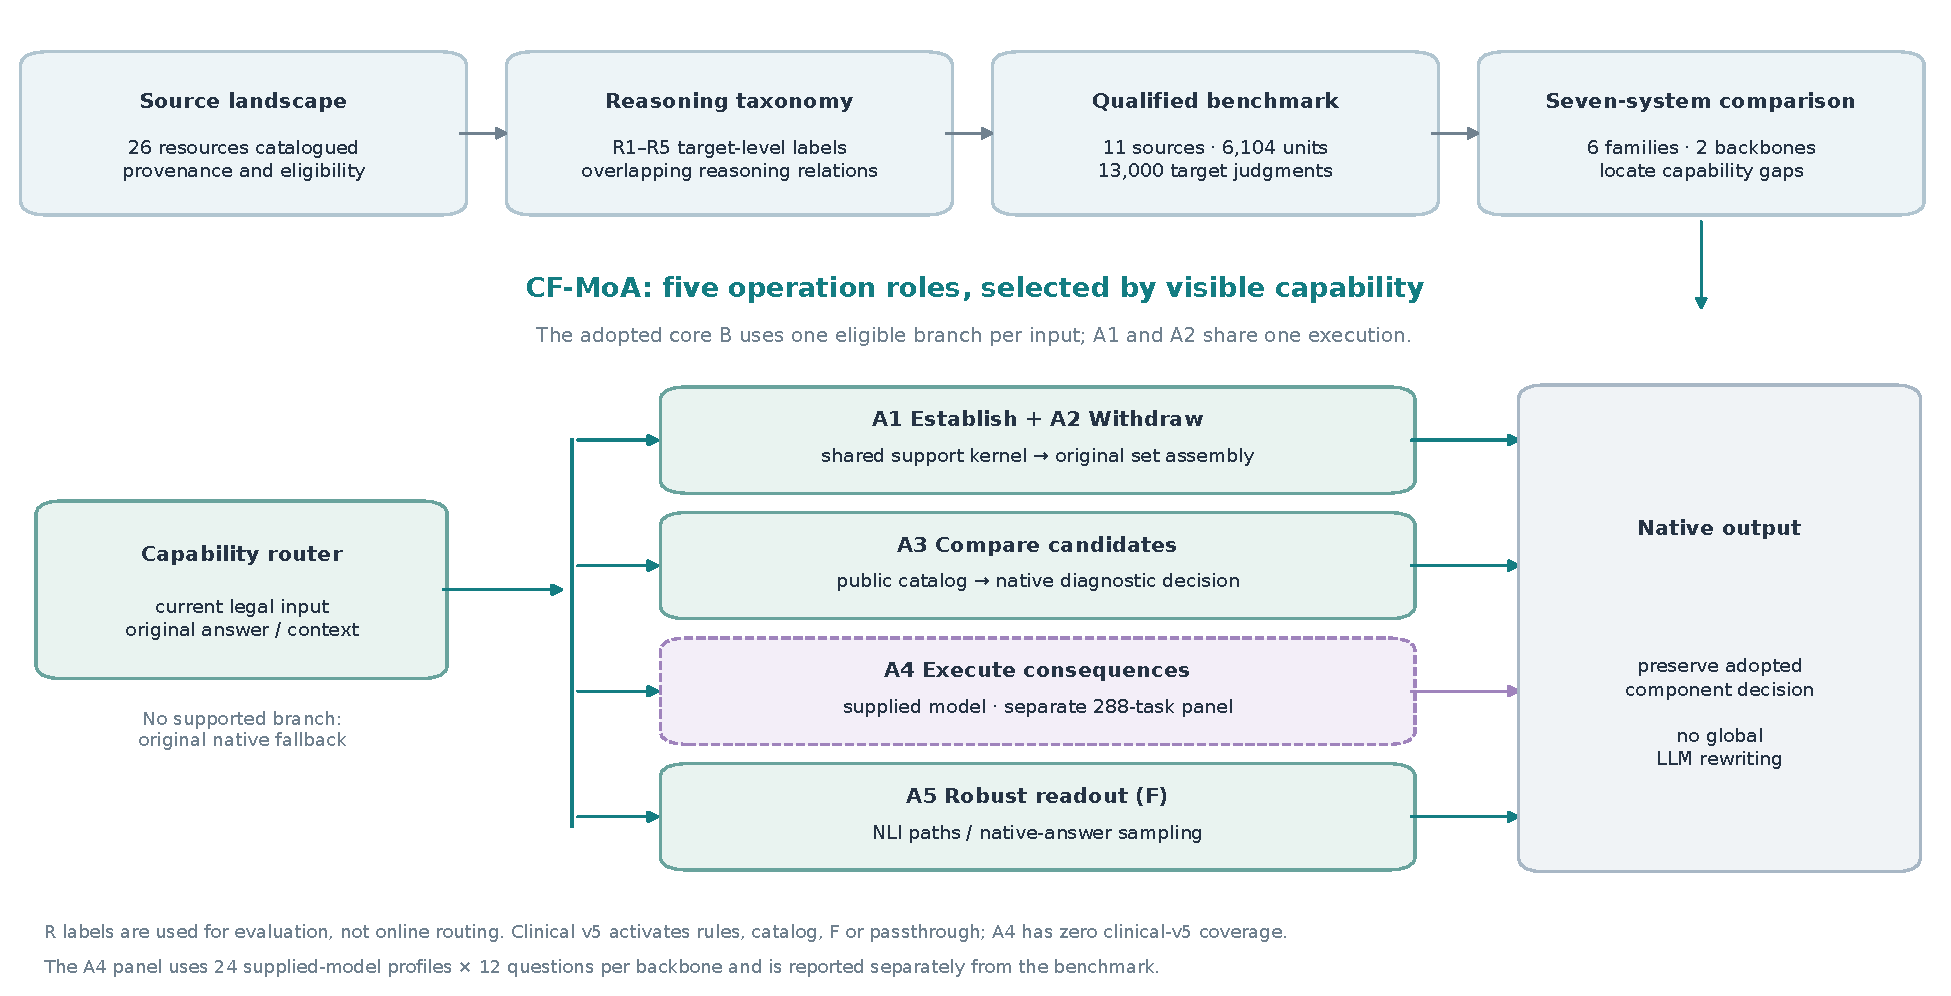
\includegraphics[width=\linewidth]{figures/story_map.pdf}
\caption{Proposed organizing figure: the offline resource--taxonomy--benchmark path motivates the online functional roles. The evaluated default routes by input capability. A1/A2 share one rule execution; A4 requires a supplied executable model. NLI denotes natural language inference; LLM denotes large language model. The figure does not imply that all five roles execute on every question.}
\label{fig:story}
\end{figure}

\section{Full Manuscript Structure}
A generic conference manuscript of approximately 7,000--7,500 main-text words is appropriate before venue-specific formatting. The final manuscript should develop the following sections.

\subsection{Introduction: Why Functional Organization Matters}
Begin with the practical demand to update an answer when relevant support changes and to preserve it when the target is unaffected. Explain how source-level evaluations obscure these different demands. Introduce the five-category view, the benchmark construction, the seven-system diagnosis, and the resulting agent framework in that order. End with the four contributions above. The opening should make the data and taxonomy contributions as prominent as the system improvement.

\subsection{Related Work: Four Connected Threads}
Cover medical retrieval-augmented generation (RAG), medical counterfactual and perturbation resources, agent composition, and constrained reasoning/readout. Position the evaluated implementations of MedRAG, MedRGAG, MA-RAG, MedGENIE, and TC-RAG using their primary references \citep{xiong2024medrag,li2026medrgag,wu2026marag,frisoni2024medgenie,jiang2025tcrag}. Discuss mixture-of-agents and self-consistency as related composition strategies \citep{wang2025moa,wang2023selfconsistency}. Explain how the functional roles differ from simply increasing answer samples, while using controls to identify any benefits that sampling already supplies. Prior calibration is an existing technique \citep{zhao2021calibrate}; its contribution must be measured separately from catalogue access.

\subsection{A Functional Taxonomy and Benchmark}
\textbf{Annotation unit.} Define each decision relative to a change, a target, and evidence for their relationship. Annotation fields retain the change, target, labels, rationale, supporting evidence, and what cannot be inferred. Five categories describe functional relations, not five learned classifiers.

\begin{table}[tbp]
\centering\small
\caption{Five functional categories and their corresponding design requirements. Category membership is determined offline; it is not a routing oracle.}
\label{tab:taxonomy}
\begin{tabularx}{\linewidth}{@{}lXX@{}}
\toprule
Category & Relation to the target & Agent role \\
\midrule
R1 & A changed condition establishes additional support. & A1: establish supported conclusions. \\
R2 & A previously supporting condition is invalidated. & A2: withdraw invalid support and check remaining paths. \\
R3 & Relative support among alternatives changes. & A3: re-compare a finite candidate set. \\
R4 & A downstream consequence must be derived under an evidenced relation. & A4: execute a conditional intervention model. \\
R5 & The specified target should retain its judgment under the change. & A5: preserve the target through robust native readout. \\
\bottomrule
\end{tabularx}
\end{table}

\textbf{Collection and qualification.} The source catalogue contains 26 candidate resources. Fifteen were acquired: 14 text resources and one metadata resource lacking required images. Their archive contains 55,991 comparison records, including 2,497 image-metadata records. Full-archive disposition tracking yields 109,599 reviewed target judgments, of which 77,781 judgments in 38,123 units across 11 sources are eligible. Classification eligibility and scoring eligibility are separate: missing images, ambiguous changes, invalid edits, unsupported target relations, unavailable semantic grading, and unexecuted knowledge-editing requirements can prevent evaluation.

\textbf{Frozen benchmark.} Version 5 retains all eligible R1--R4 judgments and randomly selects 450 R5 units from each of eight eligible R5 sources using recorded seeds. The union contains 6,104 units and 13,000 selected judgments from 11 sources. Its execution materialization has 13,905 unique inputs and 15,616 native scoring mappings per configuration. These counts measure different objects. The current audit reproduces the sampling and verifies that the original semantic fields of all 109,599 judgment records remain unchanged.

% Generated by scripts/build_story_assets.py from frozen audited summaries.
\begin{table}[tb]
\centering
\small
\setlength{\tabcolsep}{4pt}
\caption{Complete v5 benchmark composition by source. R1--R5 columns count units bearing each category label.}
\label{tab:story-benchmark}
\resizebox{\linewidth}{!}{%
\begin{tabular}{llrrrrrrr}
\toprule
ID & Source & Units & Judgments & R1 & R2 & R3 & R4 & R5 \\
\midrule
M01 & MedEinst & 1,780 & 2,816 & 1,780 & 0 & 680 & 0 & 0 \\
M02 & MedPIC-Bench & 167 & 182 & 96 & 75 & 10 & 0 & 0 \\
M06 & HIV causal scenarios & 13 & 13 & 0 & 0 & 0 & 13 & 0 \\
M10 & CPV-MedQA & 451 & 451 & 1 & 0 & 0 & 0 & 450 \\
M11 & Counterfactual Cultural Cues & 517 & 517 & 67 & 0 & 0 & 0 & 450 \\
M12 & FairMedQA/AMQA & 584 & 584 & 134 & 0 & 43 & 0 & 450 \\
M14 & DiversityMedQA & 454 & 454 & 0 & 4 & 0 & 0 & 450 \\
M17 & MedPerturb & 450 & 1,344 & 0 & 0 & 0 & 0 & 450 \\
M20 & MedCounterFact & 788 & 1,720 & 788 & 0 & 0 & 0 & 450 \\
M22 & MedRGB & 450 & 4,469 & 0 & 0 & 0 & 0 & 450 \\
M23 & BioRAB & 450 & 450 & 0 & 0 & 0 & 0 & 450 \\
\midrule
\textbf{Total} &  & 6,104 & 13,000 & 2,866 & 79 & 733 & 13 & 3,600 \\
\bottomrule
\end{tabular}}
\par\smallskip
\begin{minipage}{\linewidth}\footnotesize The benchmark contains 6,104 unique units and 13,000 target judgments. Category memberships overlap and must not be summed as independent units. Target judgments are distinct from the 13,905 inference inputs and 15,616 native scoring mappings per system. The separate supplied-model A4 panel is not added to this table.\end{minipage}
\end{table}


\textbf{Overlap and scoring.} R1--R5 contain 2,866, 79, 733, 13, and 3,600 units, respectively. Their 7,291 memberships are not 7,291 distinct cases; R3 is a subset of R1. Native scoring is retained and aggregated at the specified unit level. The overall mean uses all 6,104 units. Source fidelity audits do not establish independent clinical validation of all source answers. The development exposure and the small clinical R4 stratum must be visible in the experimental contract.

\subsection{Diagnosing Existing Medical Question-Answering Systems}
Present all seven formal configurations: direct Llama; all-Llama MedRGAG; intrinsic MA-RAG with Qwen, eight solver candidates and at most four rounds; MedRAG with Llama and repaired structured output; MedRAG with Qwen and its original output protocol; MedGENIE v2 with Llama; and typed-control-v2 TC-RAG with Qwen. These are seven configurations from six method families, not seven wholly distinct algorithms.

All use the same frozen evaluation scope. The best baseline score on R1 is 31.44\%, and the best on R3 is 30.42\%, despite overall scores ranging from 47.35\% to 51.61\%. These are native task scores within functionally annotated subsets, not pure measurements of isolated cognitive operations. Error analysis should distinguish inaccessible candidate answers, invalid native mappings, support-scope mistakes, and upstream evidence limitations. This diagnosis motivates specialized processing without attributing every error to counterfactual reasoning alone.

\subsection{CF-MoA: Five Operational Roles}
Define an agent by its functional input--operation--output contract, allowing heterogeneous internal implementations. The evaluated default is \texttt{adopted\_B\_five\_operations\_v1}. It preserves successful historical components and applies the following priority order:
\begin{enumerate}
\item Diagnosis-format inputs use A3's public 49-diagnosis catalogue with six scoring orders, existing calibration, and native answer mapping.
\item Inputs eligible for the adopted rule head use A1/A2 through one fact extraction and one shared three-valued rule execution. Positive support can be added; contradicted support can be withdrawn while valid independent paths are retained.
\item Inputs with a complete supplied executable model use A4's local intervention patch and the numerical executor.
\item Other supported single-answer, robustness, and relation inputs with available original messages use A5's adopted task-specific sampling and consensus method F.
\item Remaining inputs retain the original complete native answer.
\end{enumerate}
Only current legal input, authorized evidence, initial same-input answers where required, and declared capabilities are available online. Gold answers, offline R labels, hidden paired endpoints, and source identifiers are not routing shortcuts.

Full v5 routes 3,560 inputs through the catalogue, 123 through the rule branch, 10,178 through F, and 44 through passthrough per backbone. A4 has zero activations in this clinical benchmark and is evaluated in a separate supplied-model panel. Internal aggregation exists within the catalogue/F branches. The default is a sparse capability-routed composition, not an all-agent debate followed by a new generative judge. A1 and A2 share a kernel; their separate operational effects are tested by ablation.

The original five-agent design also sought complementary multi-expert evidence aggregation. Those variants were actually implemented and tested. Their weaker development results explain retention of the sparse default, but do not establish a general claim that collaboration cannot help. The later candidate-with-rationales verifier is an optional extension, not the definition of CF-MoA.

\subsection{Experimental Design}
Separate three evidence scopes: the complete benchmark system comparison; terminal-head portability across seven configurations on R1--R3; and operation-specific controls or additional component checks. The full default system was evaluated on the two MedRAG backbones, not all seven baseline pipelines. Head results combine actual terminal scoring with exact-request reuse and, for rule facts, documented offline combinations with seven saved answer sets.

Use the recorded paired bootstrap with 5,000 resamples over 4,766 families for full-system overall differences. Pair metrics use their own family sets. Intervals describe the exposed development scope and are not adjusted for development selection. Retain all unavailable outputs in their declared denominators. Report extra resources and calls; the seven configurations and CF-MoA do not form a budget-matched algorithm experiment.

\section{Verified Results to Foreground}
\subsection{Complete Benchmark: Seven Baselines and Two CF-MoA Instantiations}
% Generated by scripts/build_story_assets.py from frozen audited summaries.
\begin{table}[tb]
\centering
\small
\setlength{\tabcolsep}{4pt}
\caption{Complete v5 comparison of seven baseline configurations and two CF-MoA core instantiations. Scores are percentages of native-unit means.}
\label{tab:story-systems}
\resizebox{\linewidth}{!}{%
\begin{tabular}{llrrrrrr}
\toprule
System & Backbone & ALL & R1 & R2 & R3 & R4 & R5 \\
\midrule
Direct & Llama & 48.10 & 30.04 & 8.86 & 17.87 & 38.46 & 65.70 \\
MedRGAG & Llama & 48.81 & 31.33 & 7.59 & 24.69 & 53.85 & 65.88 \\
MA-RAG & Qwen & 51.61 & 26.73 & 34.18 & 8.59 & 38.46 & 73.37 \\
MedRAG & Llama & 48.20 & 27.84 & 29.11 & 30.42 & 53.85 & 65.28 \\
MedRAG & Qwen & 47.35 & 28.58 & 41.77 & 25.24 & 53.85 & 63.42 \\
MedGENIE & Llama & 48.02 & 29.94 & 18.99 & 21.42 & 61.54 & 65.15 \\
TC-RAG & Qwen & 49.43 & 31.44 & 29.11 & 28.92 & 30.77 & 66.17 \\
\midrule
\textbf{CF-MoA (B)} & Llama & 58.29 & 44.63 & 48.10 & 53.21 & 53.85 & 68.84 \\
\textbf{CF-MoA (B)} & Qwen & 59.36 & 46.62 & 58.23 & 60.03 & 23.08 & 68.79 \\
\bottomrule
\end{tabular}}
\par\smallskip
\begin{minipage}{\linewidth}\footnotesize Each row covers 13,905 inputs. ALL uses 6,104 non-reference units; R1--R5 use 2,866, 79, 733, 13, and 3,600 units. Categories overlap. These are complete system comparisons with different resources and inference budgets. Llama: Llama-3.1-8B-Instruct; Qwen: Qwen3-8B. The two MedRAG baselines retain their selected output configurations. All values describe the exposed development benchmark.\end{minipage}
\end{table}

The adopted default reaches 58.29\% with Llama and 59.36\% with Qwen. Relative to its corresponding MedRAG configuration, the improvements are 10.0934 and 12.0129 percentage points (pp), with paired family 95\% intervals of [8.9580, 11.2340] and [10.9177, 13.1510] pp. Both exceed the highest of the seven baseline overall scores, 51.61\%; differences to that value are 6.68 and 7.75 pp. This is a descriptive system comparison under shared scoring, with differing resources and inference budgets.

Table~\ref{tab:story-systems} retains every category. MA-RAG remains stronger on R5 and MedGENIE on the small R4 stratum. In particular, Qwen CF-MoA falls from 7/13 to 3/13 on clinical R4. The separate physiological execution panel must not replace that row. The overall gains support the complete system; they do not imply category-wise dominance.

\subsection{Updating and Preserving Judgments}
% Generated by scripts/build_story_assets.py from frozen audited summaries.
\begin{table}[tb]
\centering
\small
\setlength{\tabcolsep}{4pt}
\caption{Maintaining and changing answers appropriately: both endpoints must be correct.}
\label{tab:story-pairs}
\resizebox{\linewidth}{!}{%
\begin{tabular}{llll}
\toprule
Backbone & System & Maintain & Respond \\
\midrule
Llama & MedRAG (C0) & 4,005/6,838 (58.57\%) & 13/1,780 (0.73\%) \\
Llama & CF-MoA (B) & 4,440/6,838 (64.93\%) & 347/1,780 (19.49\%) \\
Qwen & MedRAG (C0) & 3,528/6,838 (51.59\%) & 27/1,780 (1.52\%) \\
Qwen & CF-MoA (B) & 4,460/6,838 (65.22\%) & 360/1,780 (20.22\%) \\
\bottomrule
\end{tabular}}
\par\smallskip
\begin{minipage}{\linewidth}\footnotesize Counts and percentages use 6,838 maintain pairs and 1,780 respond pairs. Endpoints are inferred independently; pair relations are used only for evaluation. Pairs may share endpoints or families. All planned pairs remain in the denominator.\end{minipage}
\end{table}

Both-correct pair evaluation connects directly to the functional aim: answering the changed and reference endpoints correctly, with each endpoint answered independently. On 1,780 response pairs, Llama improves from 13 to 347 correct pairs and Qwen from 27 to 360. On 6,838 preservation pairs, the corresponding counts increase from 4,005 to 4,440 and from 3,528 to 4,460. Improvements are positive in all four recorded paired family intervals. Response accuracy remains near 20\%, leaving substantial scope for improvement.

\begin{figure}[tbp]
\centering
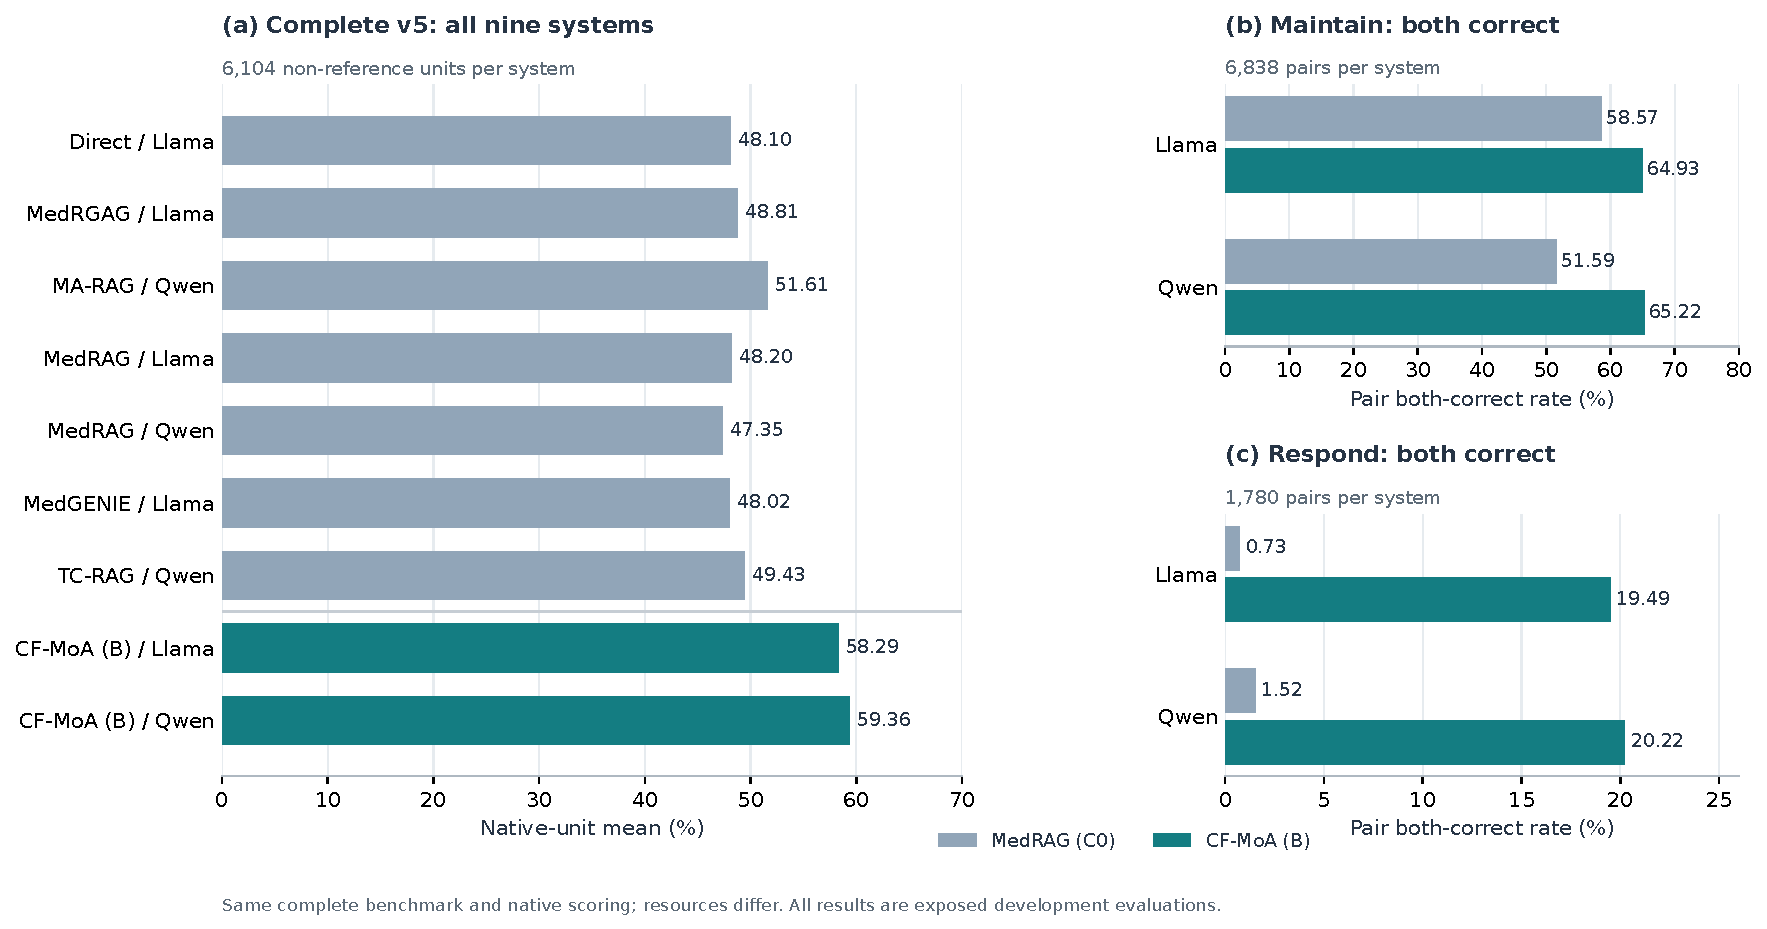
\includegraphics[width=\linewidth]{figures/story_system_results.pdf}
\caption{Complete-scope evidence prioritized for the paper: overall native unit scores and preservation/response pair correctness. Pair endpoints are independently answered. Overall and pair denominators differ; categories and pairs are not independent datasets.}
\label{fig:systems}
\end{figure}

\subsection{Breadth Across Seven Systems}
The seven-system head experiments give 21 positive before/after results: R1 gains range from 14.83 to 19.12 pp, R2 from 16.46 to 29.11 pp, and R3 from 18.69 to 35.20 pp. Use the complete seven-row table and three-panel plot already produced for the previous manuscript. The category denominators are 2,866, 79, and 733; the 3,678 memberships correspond to 2,941 unique units. These experiments establish terminal-head applicability within the evaluated systems, not seven complete five-role CF-MoA evaluations.

\subsection{Mechanisms and Necessary Controls}
\textbf{Support operations.} On all 123 rule-capability inputs, default correct counts are 69 and 71. Disabling addition reduces them to 43 and 48; disabling removal reduces them to 53 and 60. This tests two operations within a shared kernel. On the historical 79-unit R2 panel, a constant-None control is better in aggregate than every corresponding head, but fails on all nine remaining-support cases; heads recover two to six of those cases. Present both outcomes to explain why preserving surviving support is distinct from exploiting a dominant label.

\textbf{Candidate accessibility.} Across the seven configurations on 680 diagnosis inputs, average correctness is 20.97\% for original answers, 45.44\% for a single catalogue-constrained decision, 46.47\% for uncalibrated six-order voting, and 46.13\% for calibrated voting. Catalogue access/readout supplies most of the observed benefit. Calibration is not uniformly beneficial. Of 1,272 repaired configuration--case instances, 95.05\% had an originally unmapped or otherwise invalid answer; this is not evidence that every repair reflects newly acquired clinical knowledge. On an earlier 40-case development panel, name normalization yielded 15/40 and 11/40, while patient-informed catalogue re-decision yielded 18/40 on both backbones. Those adopted readout protocols differ in reasoning allowance; the comparison supports a process improvement beyond name normalization, not an equal-budget isolated effect.

\textbf{Consequence execution.} On 24 new supplied-model physiological profiles with 12 questions each, the local-patch branch achieves 288/288 jointly correct numerical outputs on both backbones. A same-tool full-plan comparator achieves 270/288 and 222/288; the patch-without-intervention control achieves 67/288 on this metric. This is bounded intervention-execution evidence under provided model/state assumptions. These are simulator profiles, not new clinical patients or additional v5 cases.

\textbf{Preservation.} Historical F improves the weighted both-correct score over 208 units from 60.19\% to 65.90\% and from 59.17\% to 66.47\%. The 208 units comprise 64 development, 128 extension, and 16 post-freeze new units. On the new 16-unit component check, single-answer counts improve from 11 to 12 and from 12 to 13 both-correct pairs. Against ordinary five-sample majority on the older 192 units, increments are only 0.52 and 1.56 pp. Keep that comparator so the full gain is not attributed solely to a new aggregation mechanism.

\subsection{Why the Default Remains Sparse}
On the historical 121-input development panel, B has 87/82 correct inputs on the two backbones, while a completed generative aggregation variant including experimental A1 has 79/74. Native overall scores over 74 units are 70.27/64.41\% for B and 63.06/54.05\% for that aggregation. This is an informative architectural comparison on its own scope. It does not prove multi-agent collaboration is universally inferior.

Preserve all six full-v5 arms in a secondary results table: original C0, adopted B, candidate-only verification, verification with rationales, the old pool plus three samples, and joint selection. The rationale extension changes the B score by $-1.81$ pp on Llama and $+0.93$ pp on Qwen. B is the same previously adopted identity on both backbones; do not assemble a new method by selecting the best later arm separately for each backbone.

\section{Figures, Tables, and Evidence Placement}
\begin{table}[tbp]
\centering\small
\caption{Planned presentation hierarchy. Supplementary placement does not remove controls from the evidential record.}
\begin{tabularx}{\linewidth}{@{}lXX@{}}
\toprule
Placement & Evidence & Purpose \\
\midrule
Main figure 1 & Construction and five-role architecture & Connect taxonomy and operational design. \\
Main tables 1--2 & Category definitions and source composition & Make the benchmark contribution explicit. \\
Main results & Complete nine-row comparison and pair results & Establish full-system improvement. \\
Breadth figure & All 21 seven-system head comparisons & Show applicability beyond the two full-system backbones. \\
Mechanism table & Add/remove, single-catalogue, constant-None & Distinguish system gains from component attribution. \\
Separate panel & Supplied-model A4 and staged F checks & Present completed capability tests with their own denominators. \\
Appendices & Six arms, all sources, exposure, costs, aggregation and failed variants & Preserve the complete development evidence and interpretation limits. \\
\bottomrule
\end{tabularx}
\end{table}
Select complete panels that directly support the contribution, rather than subsets chosen because their scores are higher. The default system and its two backbones are retained consistently. Per-source results provide heterogeneity analysis; they do not replace the complete main table. Source collection volume is a resource contribution, not a claim that every archived record is a qualified evaluation case.

\section{Research History and Interpretation}
The actual sequence begins before the head-development report. The initial September 8 request explicitly sought functional relabelling of existing medical benchmark problems while preserving their questions and scoring. Collection and early review led through earlier evaluation versions to full-archive qualification and v5. Medical RAG failures and task-specific diagnostics motivated the head studies during September 14--18. The September 21 five-agent plan introduced operational roles, routing, and evidence aggregation. Subsequent experiments explored independent experts and generative aggregation before retaining the adopted five-operation B on September 23. Later full-v5 six-arm evaluation and September 28 closeout supply the complete system evidence.

Two detailed retrospective reports preserve the iterative path: the R1--R5 report contains 148 stages, and the CF-MoA report continues through the full-v5 closeout. They are complemented by data construction, classification, baseline, and component master records. The proposed paper orders these facts by research question, design, and evidence. It does not portray the work as a single preregistered linear experiment.

Earlier world-model and paired-adapter studies belong in a development appendix when they explain input-contract or design decisions. Their different data scopes and information permissions preclude mixing their favorable scores into the v5 main table. Unsuccessful independent A1, supervised preservation, and aggregation attempts remain historical evidence rather than being recast as adopted components.

\section{Limitations and Completion Boundary}
The paper should state the development exposure, overlapping categories, source imbalance, limited clinical R4 size, shared A1/A2 implementation, conditional A4 coverage, and differing computation/resources. The final composed system has not received a new-family independent confirmation or a second independent F-pool replication. Earlier completed component checks retain their own status and should not be erased by that limitation. No clinician inter-annotator agreement or clinical deployment validation is claimed.

The benchmark is assembled and re-annotated from existing sources, with a traceable qualification process. Source fidelity does not certify all medical truth. The framework supplies five functional roles, but its evaluated default does not establish an extra gain from simultaneous five-agent deliberation. The conclusion can therefore be strong and specific: functional organization yields a useful benchmark and an effective evaluated system, while its individual mechanisms have identifiable coverage and limits.

\section{Reproduction and Next Writing Step}
The framework package contains frozen audit inputs with SHA-256 hashes, a deterministic table/figure script, the generated CSV and native LaTeX tables, two vector figures, this source, and its compiled PDF. Rendering requires no model, grader, or graphics processing unit. The existing seven-head and six-arm scripts remain available in the preceding delivery. Data values, labels, membership, and original experiment artifacts are unchanged.

The next writing step is to expand this framework into the full manuscript: lead with taxonomy and construction, introduce baseline diagnosis, present CF-MoA's adopted design, and use the complete system and mechanism panels above. The prior full manuscript is retained as a source of checked prose and references; it has not silently been relabelled as the completed new paper.

\bibliographystyle{plainnat}
\bibliography{references}
\end{document}
